%%%%%%%%%%%%%%%%%%%%%%%%%%%%%%%%%%%%%%%%
%% MCM/ICM LaTeX Template %%
%% 2026 MCM/ICM           %%
%%%%%%%%%%%%%%%%%%%%%%%%%%%%%%%%%%%%%%%%
\documentclass[12pt]{article}
\usepackage{geometry}
\geometry{left=1in,right=0.75in,top=1in,bottom=1in}

%%%%%%%%%%%%%%%%%%%%%%%%%%%%%%%%%%%%%%%%
% Replace ABCDEF in the next line with your chosen problem
% and replace 1111111 with your Team Control Number
\newcommand{\Problem}{A}
\newcommand{\Team}{2620586}
%%%%%%%%%%%%%%%%%%%%%%%%%%%%%%%%%%%%%%%%

\usepackage{newtxtext}
\usepackage{amsmath,amssymb,amsthm}
\usepackage{newtxmath} % must come after amsXXX
\usepackage{float}
\usepackage[pdftex]{graphicx}
\usepackage{xcolor}
\usepackage{fancyhdr}
\lhead{Team \Team}
\rhead{}
\cfoot{}

\newtheorem{theorem}{Theorem}
\newtheorem{corollary}[theorem]{Corollary}
\newtheorem{lemma}[theorem]{Lemma}
\newtheorem{definition}{Definition}

%%%%%%%%%%%%%%%%%%%%%%%%%%%%%%%%
\begin{document}
\graphicspath{{.}}  % Place your graphic files in the same directory as your main document
\DeclareGraphicsExtensions{.pdf, .jpg, .tif, .png}
\thispagestyle{empty}
\vspace*{-16ex}
\centerline{\begin{tabular}{*3{c}}
	\parbox[t]{0.3\linewidth}{\begin{center}\textbf{Problem Chosen}\\ \Large \textcolor{red}{\Problem}\end{center}}
	& \parbox[t]{0.3\linewidth}{\begin{center}\textbf{2026\\ MCM/ICM\\ Summary Sheet}\end{center}}
	& \parbox[t]{0.3\linewidth}{\begin{center}\textbf{Team Control Number}\\ \Large \textcolor{red}{\Team}\end{center}}	\\
	\hline
\end{tabular}}
%%%%%%%%%%% Begin Summary %%%%%%%%%%%

\begin{center}
\textbf{\LARGE On a Preliminary Model for Smartphone Battery Power Consumption}
\end{center}

\begin{center}
\textbf{Summary}
\end{center}

Smartphones are playing an increasingly important role in our daily lives. Although many past studies have established various models regarding individual components, people still lack a comprehensive understanding or theoretical model of their behaviors regarding power consumption. In this paper, we establish a comprehensive mathematical model for smartphone power consumption based on studies on individual components, and administered a simple prediction on the State-of-Charge (SOC) and remaining drainage time of a smartphone battery.

The outline of our research is to independently consider the behaviors of components, then combine them. We consider the following components: screen, processing units (CPU and GPU), network modules, speakers, peripherals (camera and microphone), and battery internal resistance loss. We consider solid-founded physical and chemical principles, such as the Arrhenius equation, Nernst equation, Fourier's law, and Newton's law of cooling, to establish our model.  

Subsequently, we combine all those factors. In the past studies, various formulas were proposed, and we extract the relationships between variables, further examine the exact values of most undetermined constants, and form a complete model. Due to confidential reasons and technical limitations, we approximate some undetermined constants basing on typical values and real-world experience. In light of these, we conduct computer simulations to verify the accuracy of our model. 

After a general simulation, we delete different factors from our program one by one to compare their contributions to the total power consumption. Next, we examine how the model changes under different changes in parameters. Finally, we provide practical recommendations for different entities to optimize battery performance and longevity.

Overall, through simplifying scenarios and establishing reasonable assumptions, we manage to build a model that can, to a certain extent, predict the SOC value and remaining drainage time of a smartphone battery, reflecting the current power consumption, and hence offer suggestions for improvement.

\textbf{Keywords:} Smartphone Battery, Power Consumption Model, State-of-Charge (SOC), Thermal Effects, Battery Degradation

%%%%%%%%%%% End Summary %%%%%%%%%%%

%%%%%%%%%%%%%%%%%%%%%%%%%%%%%%
\clearpage
\pagestyle{fancy}
% Uncomment the next line to generate a Table of Contents
%\tableofcontents
\newpage
\setcounter{page}{1}
\rhead{Page \thepage\ }
%%%%%%%%%%%%%%%%%%%%%%%%%%%%%%

\tableofcontents 
\newpage

\section{Introduction}

\subsection{Background}

\quad\, In our modern everyday life, lithium batteries have become an essential part of portable electronic devices, especially smartphones. As the performance of smartphones improves, so does their power consumption and our thirst for power. However, the battery capacity is always limited, thus the remaining battery energy have always been a concern for smartphone users.

However, this problem is not simple. Lithium-ion batteries, as the most commonly-used batteries in smartphones, exhibit high non-linearity and uncertainty in their discharging behaviors. Various factors, such as temperature, load conditions, and battery aging, can significantly affect the battery performance. 

In light of this, establishing the mathematical model of smartphone battery consumption is of great significance. This model should incorporate various factors that influence the power consumption, such as screen usage, network activity, processor load, peripheral usage and so on. Moreover, the model should also take into account the battery degradation over time, which affects the overall battery life and performance. In persuit of higher accuracy, this model, under ideal circumstances, should base entirely on physical and chemical principles. But in practice, due to the incomplete knowledge we are in control of, experimental data, statistical methods, and subsequently, empirical formulas are also necessary.

\subsection{Restatement of the Problem}

\quad\, Our team is required to establish a mathematical model to calculate the State-of-Charge (SOC, in percentage) and the remaining time of a smartphone battery before it is completely drained. The whole project consists of five subtasks:

\begin{enumerate}
	\item Develop a continuous-time model to predict the SOC value in percentage.
	\item Use the mentioned model to predict the time-to-empty (the time before the battery is completely drained).
	\item Use the mentioned model to compare the contribution of different factors.
	\item Examine how the model changes under different assumptions, parameters, and usage patterns.
	\item Use the mentioned model to provide practical recommendations for different entities to optimize battery performance and longevity.
\end{enumerate}

Despite the restated problems being quite clear, we still follows another logic to organize the contents below. 

\subsection{Our Work}

\quad\, First of all, we establish a theoretical model to calculate the power consumption of different components in a smartphone, including the screen, processing units (CPU and GPU), network modules, speakers, and peripherals (camera and microphone). Then, we combine these parts to form the total power consumption of the smartphone. Based on this, we can calculate the SOC value and the remaining drainage time.

Then, we used computer simulations to verify the accuracy of our theoretical model. After a general simulation, we deleted different factors from our program one by one to compare their contributions to the total power consumption. Next, we examined how the model changes under different assumptions, parameters, and usage patterns. Finally, we provided practical recommendations for different entities to optimize battery performance and longevity.

There might be inaccuracies, even fallacies in our model due to technical limitations, insufficient knowledge, and lack of experimental data. We have listed these limitations at the end of the paper. The strengths of our paper are also summarized there.

Here is a brief overview of our work, in the form of a flowchart.

\begin{figure}[H]
	\centering
	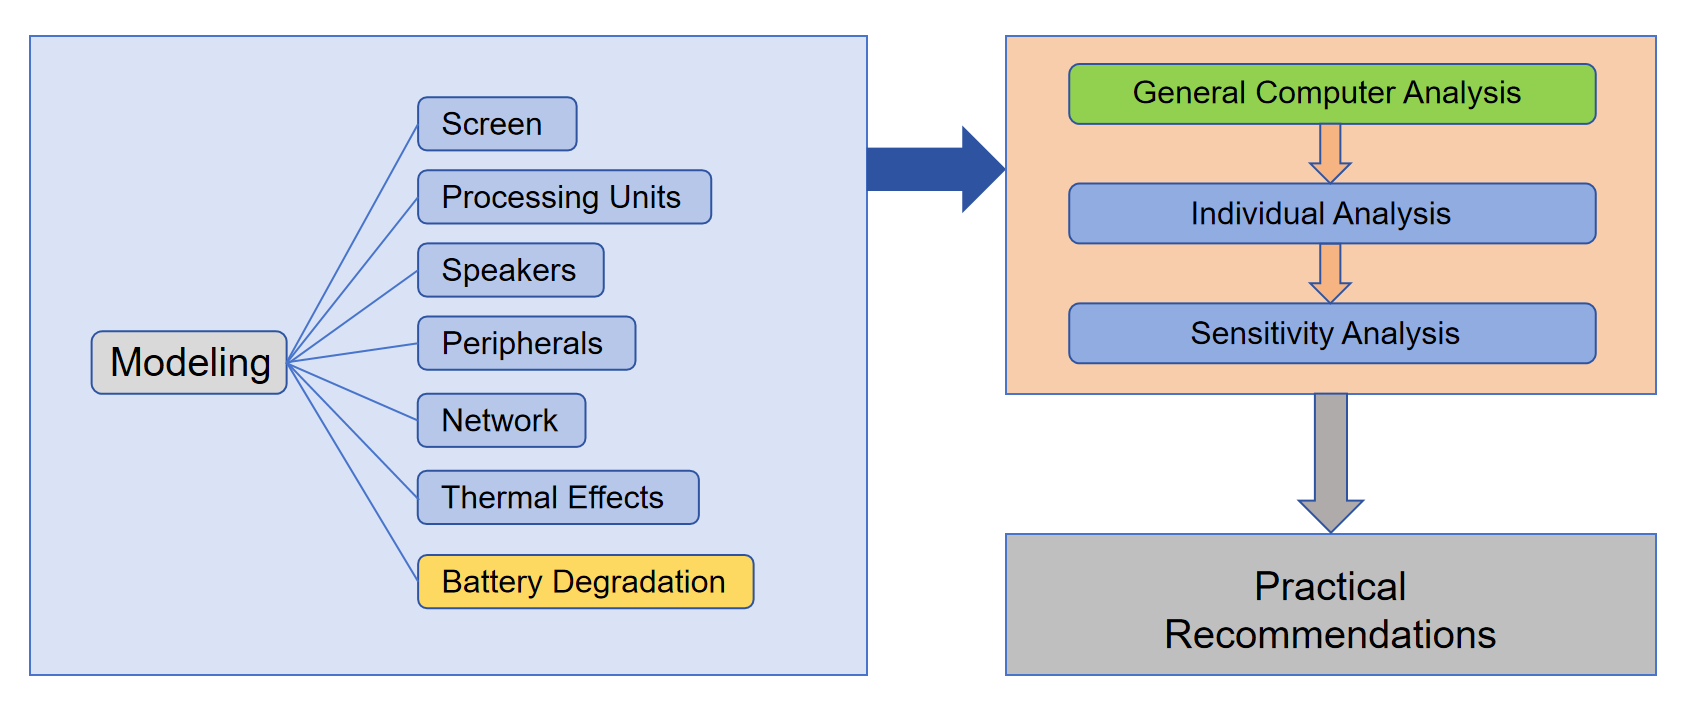
\includegraphics[width=0.8\textwidth]{workflow.png}
	\caption{Flowchart of our Work}
	\label{fig:force_here}
\end{figure}

The assumptions and justifications we use are listed in the corresponding subsections respectively. 

\section{Notations}

\quad\, The notations for most variables we use in this paper are listed below. All variables are real numbers unless otherwise specified, here we do not include any indices or superscripts, which are further explained in the corresponding contexts. Also, these meanings may be restated in the contexts for the convenience of the reader. We use SI units unless specified.

\begin{center}
\begin{tabular}{c|cc}
	\hline
	Symbol & Meaning & Unit \\
	\hline
	(SOC) & State of charge & \% \\
	$E$ & Energy / Battery capacity & J / Wh or Ah \\
	$P$ & Power & W \\
	$t$ & Time & s \\
	$T$ & Temperature & K \\
	$U$ & Voltage & V \\
	$\mathcal E$ & Electromotive force & V \\
	$I$ & Current & A \\
	$f$ & Frequency & Hz \\
	$K$ & Equilibrium constant & - \\
	$k$ & Rate constant / Thermal conductivity & - / W/(m$\cdot$K) \\
	$Q$ & Reaction quotient / Heat & - / J \\
	$q$ & Heat transfer rate & W \\
	$A$ & Area & m$^2$ \\
	$C$ & Capacitance & F \\
	$c$ & Concentration / Specific heat capacity & mol/m$^3$ / J/(kg$\cdot$K) \\
	$m$ & Mass & kg \\
	$Z$ & \textit{Complex} impedance & $\Omega$ \\
	\hline
\end{tabular}
\end{center}

The scientific constants we use are listed below.

\begin{center}
\begin{tabular}{c|c}
	\hline
	Symbol & Meaning \\
	\hline
	$k_\mathrm B$ & Boltzmann constant \\
	$R$ & Universal gas constant \\
	$F$ & Faraday constant \\
	\hline
\end{tabular}
\end{center}

Unless marked by a pair of parentheses, the input value of all functions only include the first monomial (not separated by a dot product) or fraction after the function name (+/- sign included). For example, $\exp -a/b$ means $\mathrm e^{-a/b}$, $\exp ab+c$ means $\mathrm e^{ab}+c$ but not $\mathrm e^{ab+c}$, and $\exp a/b\cdot c$ means $\mathrm e^{\frac{a}{b}}\cdot c$ but not $\mathrm e^{\frac{a}{b}\cdot c}$. Formats for fractions have also been adjusted for better readability; for example, $a/bc=\frac{a}{bc}$ is written instead as $a/(bc)$. Moreover, variable names with 2 or more letters are written within a pair of parentheses for better readability; for example, SOC is written as (SOC). The notation $\log$ denotes the natural logarithm.

\section{Theoretical Model}

\subsection{Overview}

\noindent \textbf{Assumption 3.1-1} \quad The remaining drainage time can be estimated using the average power consumption over the past period, from full charge to the current time ($t=0$ to $t=t_0$). 

\noindent \textbf{Justification 3.1-1} \quad By averaging the power consumption over a recent period, we can obtain a reliable estimate of the current usage pattern, which can be used to predict the remaining drainage time.
\\
\par We generally consider the following factors: screen, processing units, network, speakers, peripherals (camera, microphone, etc.), and battery internal resistance loss. Thus, the total power consumption is given by

\begin{eqnarray}
	& P_\mathrm{total}=\frac{\mathrm dE}{\mathrm dt} \\
	% 屏幕、电源自身、处理器、网络、发声、外设
	& P_\mathrm{total}=P_\mathrm{screen}+P_\mathrm{processor}+P_\mathrm{network}+P_\mathrm{sound}+P_\mathrm{peripherals}+P_\mathrm{battery\,loss}
\end{eqnarray}

The goal is to solve
\begin{equation}
	(\mathrm{SOC})_{t_0,N}=\left(\frac{(\mathrm{Energy\,left\,in\,battery})}{E_N}\right)\times 100\%=\left(\frac{E_N-\int_0^{t_0} P_\mathrm{total}\mathrm dt}{E_N}\right)\times 100\%
\end{equation}
and
\begin{equation}
	t_\mathrm{remain}=\frac{E_0-\int_0^{t_0} P_\mathrm{total}\mathrm dt}{t_0^{-1}\int_0^{t_0}P_\mathrm{total}\mathrm dt}.
\end{equation}

\subsection{Screen}

\noindent \textbf{Assumption 3.2-1} \quad We only consider the OLED screens.

\noindent \textbf{Justification 3.2-1} \quad OLED screens are widely used in modern smartphones due to their superior display quality compared to traditional LCD screens, which displays a trend of OLED becoming the mainstream.

\noindent \textbf{Assumption 3.2-2} \quad The thermally-stimulated migration rate is proportional to the carrier mobility.

\noindent \textbf{Justification 3.2-2} \quad The thermally-stimulated migration rate affects the movement of charge carriers within the OLED material, which in turn influences the carrier mobility. Under the condition of constant electric field and concentration of carriers, this proportionality can be assumed.
% 何意味，真的感觉自己在写学术垃圾（）

\noindent \textbf{Assumption 3.2-3} \quad The ambient lighting in one day follows a trigonometric function.

\noindent \textbf{Justification 3.2-3} \quad The ambient lighting varies periodically throughout the day, with peaks during daylight hours and troughs during nighttime. A trigonometric function can largely capture this periodic behavior.

\noindent \textbf{Assumption 3.2-4} \quad The brightness of the screen is proportional to the ambient lighting.

\noindent \textbf{Justification 3.2-4} \quad Users often adjust the screen brightness based on the surrounding ambient lighting to ensure optimal visibility and reduce eye strain. And for the proportionality, see work [1].

\subsubsection{Basic Model}

\quad \, First of all, we need to consider the mechanism of OLED screens. OLED screens work by passing current through organic compounds that emit light when energized. The current consists of electrons and holes (we summarize them as "carriers") that recombine to produce photons. The efficiency of this process is influenced by temperature. Then we may construct our model as follows.

According to the definition of power, we have

\begin{equation}
	P\propto \eta\cdot J\cdot U
\end{equation}
where $\eta$ is the efficiency (seen as a constant), $J$ is the current density, and $U$ is the voltage. Moreover, by Arrhenius equation, the carrier mobility, or the number of carriers whose energy exceeds the activation energy, is given by
\begin{equation}
	\mu(T)=\mu_0 \exp{-\frac{E_\mathrm{a}}{k_\mathrm B T}}
\end{equation}
where $\mu_0$ is a constant, $E_\mathrm{a}$ is the activation energy, $k_\mathrm B$ is the Boltzmann constant, and $T$ is the temperature in Kelvin. Thus, under stable illumination conditions when $P,\,J$ are constants, we have
\begin{equation}
	U\propto U_0\exp{\frac{E_\mathrm{a}}{k_\mathrm B T}}
\end{equation}

Now we may assume that the thermally-stimulated active migration rate $k_{nr}$ is proportional to $\mu_(T)$, i.e.
\begin{equation}
	k_{nr}=k_0\exp{-\frac{E_\mathrm {a}}{k_\mathrm B T}}
\end{equation}

Lighting efficiency under high temperature
\begin{equation}
	\eta=\frac{k_r}{k_r+k_{nr}}=\frac{1}{1+A\exp{-E_\mathrm {a}/(k_\mathrm B T)}},\,A=\frac{k_0}{k_r}
\end{equation}
where $k_r$ is the rate of electromagnetic radiation. Here we assume $P,\,U$ are constants, so
\begin{equation}
	J\propto \eta^{-1}= 1+A\exp{-E_\mathrm {a}/(k_\mathrm B T)}
\end{equation}
hence, 
\begin{equation}
	P_\mathrm {screen}\propto \exp{\frac{E_\mathrm{a1}}{k_\mathrm B T}}\cdot\left(1+A\exp{-\frac{E_\mathrm {a2}}{k_\mathrm B T}}\right)
\end{equation}

\subsubsection{Influence of Ambient Lighting}

\quad \, Citing the works from previous scholars$\rm ^{[2]}$, we have
\begin{equation}
	P_\mathrm{screen}=a_0+(Br)(a_\mathrm RP_\mathrm R+a_\mathrm GP_\mathrm G+a_\mathrm BP_\mathrm B)
\end{equation}
where indices R, G, B denote red, green, and blue respectively; $a_0,\,a_\mathrm R,\,a_\mathrm G,\,a_\mathrm B$ are constants related to the specific screen; $P_\mathrm R,\,P_\mathrm G,\,P_\mathrm B$ are the percentages of red, green, and blue respectively; and $(Br)$ is the brightness of the screen.

According to Assumption 3.2-3 and 3.2-4, we have
\begin{equation}
	(Br)=\varepsilon L_\mathrm{amb}=\varepsilon L_0\sin{\left(\omega t+\delta\right)}+L_\mathrm{base}
\end{equation}
where $L_0$ is the maximum ambient lighting in a day, $\delta$ is a phase shift depending on the geographical location, $L_\mathrm{base}$ is the base ambient lighting, and $\varepsilon$ is the proportionality constant. When considering indoor usages, we may set $\varepsilon$ to a smaller value, or even 0.

\subsection{Network}

\noindent \textbf{Assumption 3.3-1} \quad We only consider the data transmission power consumption.

\noindent \textbf{Justification 3.3-1} \quad Data transmission is the primary function of network modules in smartphones, and it significantly contributes to power consumption. Other functions, such as idle listening or background processes, generally consume less power and can be considered negligible for the purpose of this model.

\noindent \textbf{Assumption 3.3-2} \quad We see GPS usage as a type of network activity.

\noindent \textbf{Justification 3.3-2} \quad GPS modules in smartphones rely on network connectivity to receive satellite signals and provide location services. Therefore, the power consumption associated with GPS usage can be reasonably modeled as part of the overall network activity.
\\
\par Citing the works from previous scholars$\rm ^{[3]}$, we have the following equation
\begin{equation}
	P_{\mathrm {network}}=\sum_i \alpha_{\mathrm ui}\theta_{\mathrm ui}+\alpha_{\mathrm di}\theta_{\mathrm di}+\beta
\end{equation}
where $\alpha_{\mathrm ui},\,\alpha_{\mathrm di},\,\beta$ are constants related to the specific network type, and $\theta_{\mathrm ui},\,\theta_{\mathrm di}$ are the upload and download throughputs (in Mbps) respectively. The index $i$ denote different processes.

\subsection{Processing Units}

\noindent \textbf{Assumption 3.4-1} \quad We consider only static and dynamic power consumption of the CPU.

\noindent \textbf{Justification 3.4-1} \quad Static and dynamic power consumption are the primary contributors to the overall power consumption of a CPU. Other factors, such as short-circuit power consumption and leakage power consumption, are generally less significant and can be either neglected or included in the static power consumption.

\noindent \textbf{Assumption 3.4-2} \quad We consider the CPU is equivalent in effect to a composite of multiple transistors in dynamic states.

\noindent \textbf{Justification 3.4-2} \quad For every tiny transistor in the CPU, we focus on its effect of storing charges, and thus see it as a tiny capacitor. Thus, the CPU can be modeled as a composite of multiple transistors in dynamic states.

\noindent \textbf{Assumption 3.4-3} \quad The dynamic power consumption is proportional to the voltage squared and frequency.

\noindent \textbf{Justification 3.4-3} \quad According to Assumption 3.4-2, it is very obvious that $P_\mathrm{dynamic}\propto U^2$. Furthermore, in unit time, the number of cycles of capacitors being charged and discharged is proportional to the frequency $f$. Thus, we also have $P_\mathrm{dynamic}\propto f$. 

\noindent \textbf{Assumption 3.4-4} \quad The frequency is proportional to a power function of the voltage.

\noindent \textbf{Justification 3.4-4} \quad The frequency of a CPU is determined by the clock speed, which is influenced by the voltage supplied to the CPU. By approximating using Taylor expansion, we may assume that $f\propto U^\mu$ within small variations.

\noindent \textbf{Assumption 3.4-5} \quad The formulas for GPU power consumption are similar to those for CPU.

\noindent \textbf{Justification 3.4-5} \quad CPU and GPU share similar architectures and operational principles. Therefore, the formulas for them can be considered similar in format, with differences in constants.

\subsubsection{CPU}

\begin{equation}
	P_\mathrm{CPU}=P_\mathrm{static}+P_\mathrm{dynamic}
\end{equation}

According to Assumption 3.4-3, in unit time, the dynamic power consumption is proportional to $U^2\cdot f$, i.e.
\begin{equation}
	P_\mathrm{dynamic}=\lambda U^2\cdot f
\end{equation}
where $f$ is related to $U$. Suppose 
\begin{equation}
	f=b U^\mu
\end{equation}
and the CPU utility is $\alpha$, then
\begin{equation}
	P_\mathrm{dynamic}=\alpha U^{2+\mu}b\lambda
\end{equation}
Citing the works from previous scholars$\rm ^{[4]}$, we have the static power consumption
\begin{equation}
	P_\mathrm{static}=U\left(c_1T^2\mathrm e^{c_2/T}+I_\mathrm{gate}\right)
\end{equation}
where $c_1,\,c_2$ are constants related to the specific CPU, and $I_\mathrm{gate}$ is the leakage current of the transistor gates.

\subsubsection{GPU}

Similar to CPU, we have
\begin{eqnarray}
	& P_\mathrm{GPU}=P_\mathrm{static}+P_\mathrm{dynamic} \\
	& P_\mathrm{dynamic}=\alpha' U_\mathrm{GPU}^{2+\mu'}b'\lambda' \\
	& P_\mathrm{static}=U_\mathrm{GPU}\left(c_3T^2\mathrm e^{c_4/T}+I_\mathrm{gate}'\right)
\end{eqnarray}

\subsection{Speakers}

\quad \,Citing the works from previous scholars$\rm ^{[5]}$, we have
\begin{equation}
	U_\mathrm{in,req}(L_c)=10^{\Delta L/20}U_\mathrm{ref}
\end{equation}
where $U_\mathrm{in,req}$ is the required input voltage, $L_c$ is the volume level chosen by the user, $\Delta L=L_c-L_\mathrm{ref}$ is the difference between $L_c$ and the reference volume level, and $U_\mathrm{ref}$ is the reference input voltage.

The reference level is measured under the same circumstances, and vary accordingly with the exact speakers.

And by the definition of power, the power consumption of the speaker is
\begin{equation}
	P_\mathrm{speaker}=\Re Z(f)\cdot\frac{U_\mathrm{in,req}(f)^2}{|Z(f)|^2}
\end{equation}
where $f$ is the frequency (related to time $t$), $Z(f)\in\mathbb C$ is the complex impedance of the speaker coil, symbol $\Re$ denotes the real part.

\subsection{Peripherals}

\noindent \textbf{Assumption 3.6-1} \quad We only consider the power consumption of camera and microphone.

\noindent \textbf{Justification 3.6-1} \quad Camera and microphone are the most commonly used peripherals in smartphones, and they significantly contribute to power consumption. Other peripherals, such as sensors or haptic feedback, generally consume less power and can be considered negligible.

\noindent \textbf{Assumption 3.6-2} \quad The power consumption of camera is proportional to the number of pixels and the frame rate.

\noindent \textbf{Justification 3.6-2} \quad The number of pixels determines the amount of data that needs to be processed and transmitted, while the frame rate affects the frequency of data capture and processing. Both factors directly influence the power consumption of the camera.

\noindent \textbf{Assumption 3.6-3} \quad The power consumption of microphone is proportional to the sampling rate and bit rate.

\noindent \textbf{Justification 3.6-3} \quad The sampling rate determines how frequently audio samples are captured, while the bit rate affects the amount of data that needs to be processed and transmitted. Both factors directly influence the power consumption of the microphone.

\subsubsection{Camera}

According to Assumption 3.6-2, we have
\begin{equation}
	P_\mathrm{camera}=\gamma\cdot N_\mathrm{pixels}\cdot f_\mathrm{frame}+P_\mathrm{default,camera}
\end{equation}

\subsubsection{Microphone}

According to Assumption 3.6-3, we have
\begin{equation}
	P_\mathrm{microphone}=\delta\cdot f_\mathrm{sample}b_\mathrm{bitrate}+P_\mathrm{default,microphone}
\end{equation}

\subsection{Thermal Effects}

\noindent \textbf{Assumption 3.7-1} \quad We only consider the heat generated by the processing units and the battery internal resistance.

\noindent \textbf{Justification 3.7-1} \quad The processing units and the battery internal resistance are the main sources of heat generation in a smartphone. Other components, such as the screen and network modules, generate relatively less heat and can be neglected for simplicity.

\noindent \textbf{Assumption 3.7-2} \quad We consider four key temperatures: the temperature of the processing units, the temperature of the battery, the overall phone environment temperature, and the external environment temperature.

\noindent \textbf{Justification 3.7-2} \quad These four temperatures are crucial in understanding the thermal dynamics of the smartphone. The processing units and battery temperatures directly affect their performance and longevity, while the overall phone environment temperature influences user comfort and device safety, and reflects the working condition of electronic components. The external environment temperature serves as a boundary condition for heat transfer analysis.

\noindent \textbf{Assumption 3.7-3} \quad We see the processing units as pure resistances.

\noindent \textbf{Justification 3.7-3} \quad There is no other form of energy conversion in the processing units except for heat generation due to resistance. 
\\
\par According to Joule's law and Assumption 3.7-3, the heat generated by the units can be described as 
\begin{eqnarray}
	& q_\mathrm{P.U.}=\frac{\mathrm dQ_\mathrm{P.U.}}{\mathrm dt}=U_\mathrm{P.U.}I_\mathrm{P.U.}\\
	& q_\mathrm{battery}=I_\mathrm{battery}^2r_\mathrm{i}
\end{eqnarray}
then we may use the Fourier's law to analyze the heat transfer. Suppose the effective distance between the heat source and the other components is $d$, and the effective area of heat transfer is $A$, then we have
\begin{equation}
	q_\mathrm{disp}=k_\mathrm {P.U.}A_\mathrm{P.U.}\frac{T_\mathrm{P.U.}-T_\mathrm{env}}{d}+k_\mathrm {battery}A_\mathrm{battery}\frac{T_\mathrm{battery}-T_\mathrm{env}}{d}
\end{equation}
where $k$ is the thermal conductivity of the material between the source and the overall phone environment, $T_\mathrm{source}$ is the temperature of the heat source, and $T_\mathrm{env}$ is the temperature of the phone environment, where all other components are in direct contact with.

Then, for the thermal sources, we have
\begin{eqnarray}
	& q_\mathrm {P.U.}-k_\mathrm {P.U.}A_\mathrm{P.U.}\frac{T_\mathrm{P.U.}-T_\mathrm{env}}{d}=c_\mathrm{P.U.}m_\mathrm{P.U.}\frac{\mathrm dT_\mathrm{P.U.}}{\mathrm dt} \\
	& q_\mathrm {battery}-k_\mathrm {battery}A_\mathrm{battery}\frac{T_\mathrm{battery}-T_\mathrm{env}}{d}=c_\mathrm{battery}m_\mathrm{battery}\frac{\mathrm dT_\mathrm{battery}}{\mathrm dt}
\end{eqnarray}
where $c$ is the specific heat capacity of the processing unit material, and $m$ is the mass of the processing unit. For the overall phone environment, we have
\begin{equation}
	q_\mathrm{disp}-q_\mathrm{ext}=c_\mathrm{env}m_\mathrm{env}\frac{\mathrm dT_\mathrm{env}}{\mathrm dt}
\end{equation}
where $c_\mathrm{env}$ is the overall heat capacity of the phone environment, and $q_\mathrm{ext}$ is the heat loss to the external environment, which can be modeled using Newton's law of cooling
\begin{equation}
	q_\mathrm{ext}=hA_\mathrm{phone}\frac{\mathrm d(T_\mathrm{env}-T_\mathrm{ext})}{\mathrm dt}=hA_\mathrm{phone}\frac{\mathrm dT_\mathrm {env}}{\mathrm dt}
\end{equation}
where $h$ is the overall heat transfer coefficient, $A_\mathrm{phone}=2A_\mathrm{screen}\approx A_\mathrm{P.U.}+A_\mathrm{battery}$ is the surface area of the phone, and $T_\mathrm{ext}$ is the temperature of the external environment, which we see as a constant.

\subsection{Battery Degradation}

\noindent \textbf{Assumption 3.8-1} \quad The capacity degradation of the battery is mainly caused by the loss of lithium ions in the electrolyte during charge-discharge cycles.

\noindent \textbf{Justification 3.8-1} \quad During the charge-discharge cycles, some lithium ions may become trapped in the electrode materials or form solid electrolyte interphase (SEI) layers, leading to a decrease in the number of active lithium ions available for intercalation and de-intercalation. This loss of lithium ions results in a reduction of the battery's overall capacity over time.

\noindent \textbf{Assumption 3.8-2} \quad We only consider complete draining cycles.

\noindent \textbf{Justification 3.8-2} \quad Complete draining cycles provide a standardized way to measure battery degradation. Moreover, an incomplete draining cycle can be seen as one battery with complete drainage and another battery with no drainage.

\noindent \textbf{Assumption 3.8-3} \quad The loss ratio of lithium ions in the electrolyte during charging and discharging are independent.

\noindent \textbf{Justification 3.8-3} \quad The chambers of charging and discharging reactions are separated, and the corresponding reactions can thus be considered independent.

\noindent \textbf{Assumption 3.8-4} \quad We only consider a generalized reaction
\begin{equation}
	\rm LiM(s)+ \mathit xe^- + \mathit xLi^+ \rightleftharpoons Li_{1+\mathit x}M(s)
\end{equation}
where M is the electrode material.

\noindent \textbf{Justification 3.8-4} \quad The equations for different reactions is only different by constants, which means one can multiply a constant factor to adjust the model for specific reactions. Thus the overall form of the model remains unchanged.

\noindent \textbf{Assumption 3.8-5} \quad We consider the mass of electrolyte and the anode and cathode remain constant during charge-discharge cycles.

\noindent \textbf{Justification 3.8-5} \quad Under normal circumstances, every charge-discharge cycle is very close to a complete reaction, thus the mass of electrolyte and the anode and cathode remain nearly constant.

\subsubsection{Charge-Discharge Cycles}

\quad \, By Nernst equation, we have
\begin{equation}
	\mathcal E=\mathcal E^{\circ}-\frac{RT}{nF}\log Q
\end{equation}
where $\mathcal E$ is the electromotive force, $\mathcal E^{\circ}$ is the standard electromotive force (magnitude 3.0401 V for the pair Li/Li$^+$), $R$ is the universal gas constant, $T$ is the temperature in Kelvin, $n$ is the number of moles of electrons transferred in the reaction, $F$ is the Faraday constant, and $Q$ is the reaction quotient.

Now we substitute $\mathcal E=U_\mathrm{min},$ where $U_\mathrm{min}$ is the minimum battery output voltage, and we have $Q=K$, the equilibrium constant. Thus,
\begin{equation}
	U_\mathrm{min}=\mathcal E^{\circ}-\frac{RT}{nF}\log K\Rightarrow K=\exp{\frac{nF(\mathcal E^{\circ}-U_\mathrm{min})}{RT}}
\end{equation}

We consider the total reaction
\begin{equation}
	\rm LiM(s)+ \mathit xe^- + \mathit xLi^+ \rightleftharpoons Li_{1+\mathit x}M(s)
\end{equation}
and the forward reaction (charging state), we have the equilibrium constant
\begin{equation}
	K_+=c^{-x}(\mathrm{Li^+})=\left(\frac{M(\mathrm {Li})\cdot V}{m(\mathrm{Li^+})}\right)^x
\end{equation}
where $V$ is the volume of the electrolyte. Hence, 
\begin{equation}
	m(\mathrm{Li^+})=M(\mathrm {Li})\cdot V\cdot K_+^{-\frac{1}{x}}=M(\mathrm {Li})\cdot V\cdot \exp{-\frac{nF(\mathcal E^{\circ}_+-U_\mathrm{min+})}{xRT}}
\end{equation}
If we define $1-r_+$ as the loss ratio of lithium ions in the electrolyte, then
\begin{equation}
	r_+=1-\frac{m(\mathrm{Li^+})}{m_0}=1-\frac{M(\mathrm {Li})\cdot V}{m_0}\cdot \exp{-\frac{nF(\mathcal E^{\circ}_+-U_\mathrm{min+})}{xRT}}
\end{equation}

Now we consider the reverse reaction (discharging state), we have the equilibrium constant
\begin{equation}
	K_-=c^x(\mathrm{Li^+})=\left(\frac{m(\mathrm{Li^+})}{M(\mathrm {Li})\cdot V}\right)^x
\end{equation}
Using similar methods and note that $\mathcal E^{\circ}_+=-\mathcal E^{\circ}_-$, we have
\begin{equation}
	r_-=1-\frac{M\mathrm{(Li^+)}\cdot V}{m_0}\exp {-\frac{nF(U_\mathrm{min-}+\mathcal E^{\circ}_+)}{xRT}}
\end{equation}

and the capacity after $N$ cycles is
\begin{equation}
	E_N=E_0r_+^Nr_-^N
\end{equation}

\subsubsection{Internal Resistance}

\quad \, Citing the works from previous scholars$\rm ^{[6]}$, we may use a polynomial to model the internal resistance of the battery
\begin{equation}
	r_\mathrm i=\left(x_1+x_2(\mathrm{SOC})+x_3(\mathrm{SOC})^2+x_4(\mathrm{SOC})^3\right)x_5\varphi_N\exp{\frac{x_6}{T+x_7}}
\end{equation}
where $x_i$ are constants related to the specific battery, and $\varphi_N=\varphi_0^N$ (we assume) is a coefficient related to the number of cycles.

\subsubsection{Ambient Temperature}

\quad \, The ambient temperature affects the battery degradation in two main ways: it influences the rate of chemical reactions within the battery and affects the internal resistance of the battery. 

According to the Arrhenius equation, the rate constant $k$ of a chemical reaction is given by
\begin{equation}
	k=A\exp{-\frac{E_\mathrm a}{RT}}
\end{equation}
where $A$ is the pre-exponential factor, $E_\mathrm a$ is the activation energy.
Thus, higher ambient temperatures lead to increased reaction rates, which can accelerate the degradation processes within the battery.

As for the internal resistance, we have already modeled it in Eq.(40), where an increase in temperature generally leads to a decrease in internal resistance, which can improve battery performance but may also contribute to faster degradation due to increased reaction rates.

Furthermore, if we consider the brownian motion of lithium ions, we have the diffusion coefficient
\begin{equation}	
	D=\frac{k_\mathrm BT}{6\pi \eta r}
\end{equation}
where $\eta$ is the viscosity of the electrolyte, and $r$ is the radius of the lithium ion. Higher temperatures lead to increased diffusion coefficients, which can enhance the mobility of lithium ions within the battery. This increased mobility can improve battery performance but may also contribute to faster degradation due to increased reaction rates.

Last, extreme temperatures (both high and low) can cause the SEI layer to collapse or become unstable, leading to increased lithium ion loss and accelerated capacity fade.

\section{Numerical Simulation and Results}

\subsection{Parameter Values for Short-Term Simulation}

The parameters we choose are listed below. Some values are estimated based on typical smartphone specifications, while others are derived from empirical data or literature. Those without specified units are either not convenient to express in SI (indicated with N/A) or based on SI conventions (indicated with a space) or with no unit in itself (indicated with a dash).

\subsubsection{Screen}

\begin{center}
\begin{tabular}{c|cc}
	\hline
	Parameter & Value & Unit (Only those not in SI) \\
	\hline
	$E_\mathrm{a1}$ & 0.7 & eV \\
	$E_\mathrm{a2}$ & 0.2 & eV \\
	\hline
	$P_\mathrm{R}$ & 100 & \% \\
	$P_\mathrm{G}$ & 100 & \% \\
	$P_\mathrm{B}$ & 100 & \% \\
	$(Br)$ & 75 & \% \\
	$a_\mathrm R$ & 3.399\,6 & N/A \\
	$a_\mathrm G$ & 7.050\,3 & N/A \\
	$a_\mathrm B$ & 19.508\,1 & N/A \\
	$a_0a_\mathrm R$ & 242.318\,0 & N/A \\
	$a_0a_\mathrm G$ & 293.699\,9 & N/A \\
	$a_0a_\mathrm B$ & 294.013\,9 & N/A \\
	$L_0$ & 0.01 & N/A \\
	$\omega$ & $\pi/12$ & rad/hour \\
	$\delta$ & 0 & rad \\
	$L_\mathrm{base}$ & 0.01 & N/A \\
	\hline
\end{tabular}
\end{center}

\subsubsection{Network}

\begin{center}
\begin{tabular}{c|ccc}
	\hline
	Parameter & Value & Unit (Only those not in SI) \\
	\hline
	$P_\mathrm{network}$ & 0.2 & \\
	\hline
\end{tabular}
\end{center}

\subsubsection{Processing Units}

\begin{center}
\begin{tabular}{c|cc}
	\hline
	Parameter & Value & Unit (Only those not in SI) \\
	\hline
	$\alpha$ & 0.5 & N/A \\
	$\alpha'$ & 0.5 & N/A \\
	$b$ & 1.0 & N/A \\
	$b'$ & 1.0 & N/A \\
	$\mu$ & 1 & - \\
	$\mu'$ & 1 & - \\
	$\lambda$ & 2 & N/A \\
	$\lambda'$ & 2.5 & N/A \\
	$c_1$ & 0.255\,0 & N/A \\
	$c_2$ & -374\,0 & N/A \\
	$c_3$ & 0.256\,1 & N/A \\
	$c_4$ & -374\,0 & N/A \\
	$I_\mathrm{gate}$ & $1\times 10^{-7}$ &  \\
	$I_\mathrm{gate}'$ & $8.6\times 10^{-8}$ &  \\
	\hline
\end{tabular}
\end{center}

\subsubsection{Speaker and Peripherals}

\begin{center}
\begin{tabular}{c|cc}
	\hline
	Parameter & Value & Unit (Only those not in SI) \\
	\hline
	$P_\mathrm{speaker}$ & 0.3 & \\
	$P_\mathrm{camera}$ & 0.02 & \\
	$P_\mathrm{microphone}$ & 0.1 & \\
	\hline
\end{tabular}
\end{center}

\subsubsection{Thermal Effects}

\begin{center}
\begin{tabular}{c|cc}
	\hline
	Parameter & Value & Unit (Only those not in SI) \\
	\hline
	$U_\mathrm{P.U.}$ & 3.7 & \\
	$I_\mathrm{P.U.}$ & 2.0 & \\
	$I_\mathrm{battery}$ & 0.5 & \\
	$d$ & 0.005 & \\
	$c_\mathrm{P.U.}$ & 712 & \\
	$m_\mathrm{P.U.}$ & 0.005 & \\
	$k_\mathrm{P.U.}$ & 1 & N/A \\
	$c_\mathrm{battery}$ & 900 & \\
	$m_\mathrm{battery}$ & 0.12 & \\
	$k_\mathrm{battery}$ & 2.5 & N/A \\
	% $c_\mathrm{env}$ & 900 & \\
	$m_\mathrm{env}$ & 0.06 & \\
	$A_\mathrm{phone}$ & 2$\times$ 0.011\,86 & \\
	$A_\mathrm{P.U.}$ & 2$\times$ 0.001\,75 & \\
	$A_\mathrm{battery}$ & 2$\times$ 0.000\,06 & \\
	\hline
\end{tabular}
\end{center}

\subsubsection{Miscellaneous}

For the battery internal resistance, we use the following data under $0.75C$ conditions.

\begin{center}
\begin{tabular}{c|ccccccc}
	\hline
	Discharge Rate $\backslash$ Index & 1 & 2 & 3 & 4 & 5 & 6 & 7 \\
	\hline
	0.75C & 4.834\,7 & -0.243\,7 & -0.375\,1 & -0.162\,8 & 6.057\,7 & 2.692\,1 & -0.815\,9 \\
	1.75C & 4.236\,2 & -0.276\,0 & -0.624\,8 & -0.024\,0 & 19.906\,8 & 2.725\,3 & 0.182\,2 \\
	2.75C & 3.382\,4 & -1.097\,3 & -0.366\,8 & 0.712\,6 & 23.528\,7 & 2.666\,8 & 0.094\,0 \\
	\hline
\end{tabular}
\end{center}

We set the initial temperature to be 298 K.

The sources of the data above: see works [7] to [13].

\subsection{Short-Term Simulation}

\quad \, Here we simulate the battery drainage over one cycle. We monitored the parameter $(\rm SOC)$ and temperatures of different entities during the period. The values are plotted below.

\begin{figure}[H]
	\centering
	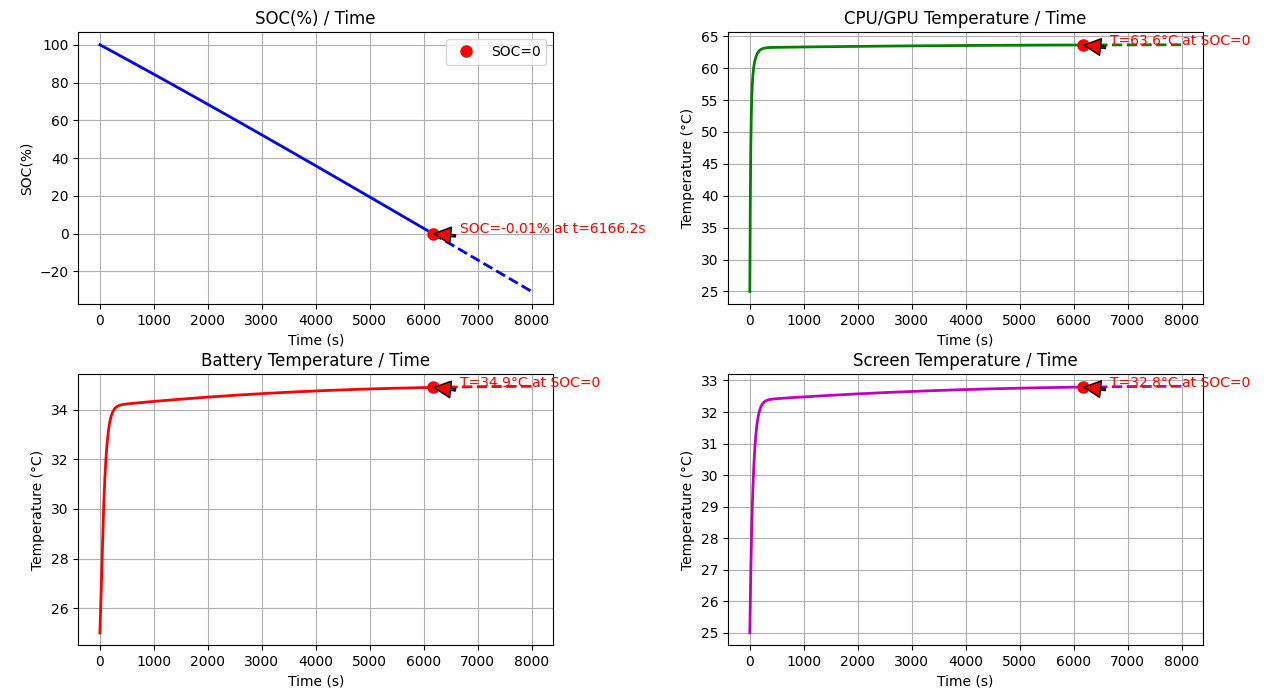
\includegraphics[width=1.0\textwidth]{It's FUCKING RAW!!!.png}
	\caption{(SOC) over Time and Temperature monitoring}
	\label{fig:force_here}
\end{figure}

We configured a high load senario, including high screen brightness, intensive CPU and GPU usages, continuous network activity, and high volume level. As shown in the figure, the battery drains from 100\% to 0\% in approximately 2 hours. The temperatures of the processing units and battery rise significantly during this period, while the overall phone environment temperature remains relatively stable due to heat dissipation.

\subsection{Long-Term Simulation}

\quad \, Here we simulate the battery degradation over 100 complete charge-discharge cycles. The values of parameters used in Eq.(40) and Eq.(42) are as follows (In consideration of the usual charging voltage 5 V, we set $U_\mathrm{min-}+U_\mathrm{min+}=5$ V, and other non-scientific constants are chosen by real-life experience):

\begin{center}
\begin{tabular}{c|c}
	\hline
	Parameter & Value \\
	\hline
	$M(\mathrm{Li})$ & 7 g/mol \\
	$m_0$ & 50 g \\
	$V$ & $2.5\times 10^{-7}$ m$^3$ \\
	$\mathcal E^{\circ}_+$ & 3.0401 V \\
	$U_\mathrm{min+}$ & 1.3 V \\
	$U_\mathrm{min-}$ & 3.7 V \\
	$R$ & 8.314 J/(mol$\cdot$K) \\
	$F$ & 96485 C/mol \\
	$T$ & 298 K \\
	$n$ & 0.35 mol \\
	$x$ & 1 \\
	\hline
\end{tabular}
\end{center}
where the $\mathcal E^{\circ}_+$ value is from the CRC Handbook of Chemistry and Physics (see [11]).

We calculate
\begin{eqnarray}
	& r_+\approx 0.997\,179\,320\,7\\
	& r_-\approx 1
\end{eqnarray}

Thus, we plot the capacity degradation over 500 complete charge-discharge cycles as follows.

\begin{figure}[H]
	\centering
	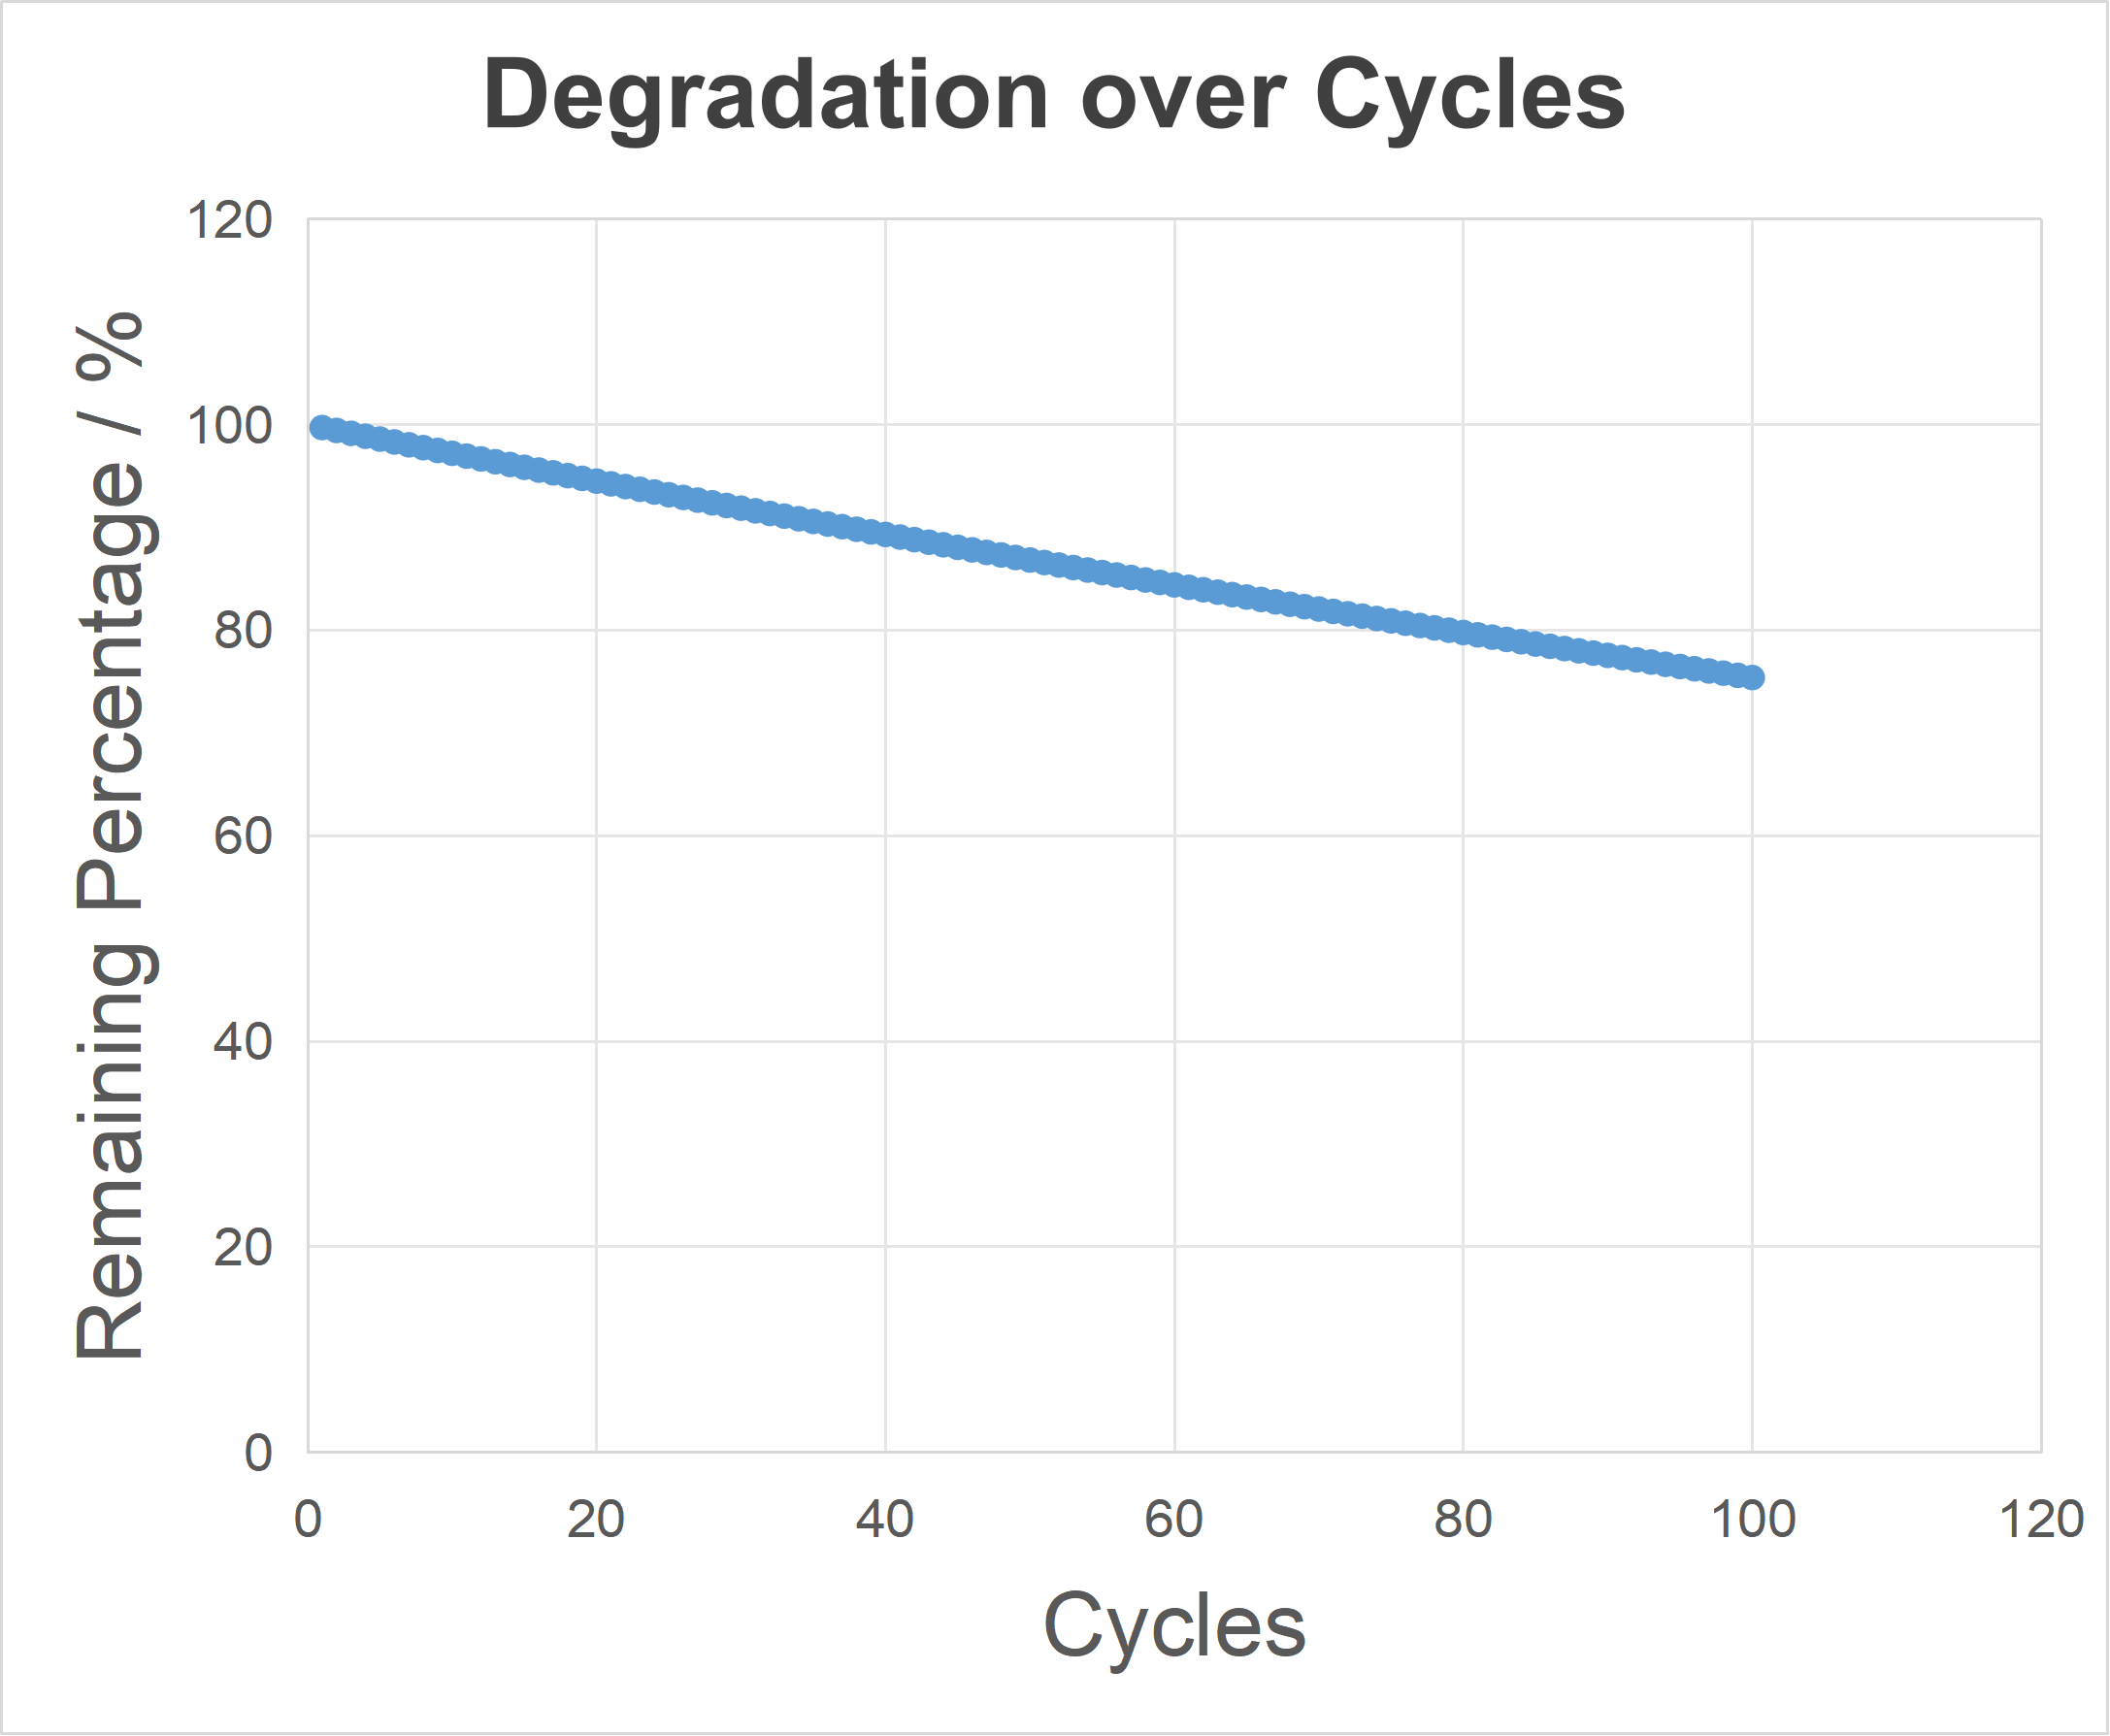
\includegraphics[width=0.6\textwidth]{degradation over cycles.png}
	\caption{Capacity Degradation over 100 Complete Charge-Discharge Cycles}
	\label{fig:force_here}
\end{figure}

After 100 complete charge-discharge cycles, the battery capacity drops to approximately 75.392\% of its original capacity.

\subsubsection{Preliminary Validation}

\quad \, We compared our simulated total power with the power measured in experiment. The results are as follows.

\begin{figure}[H]
	\centering
	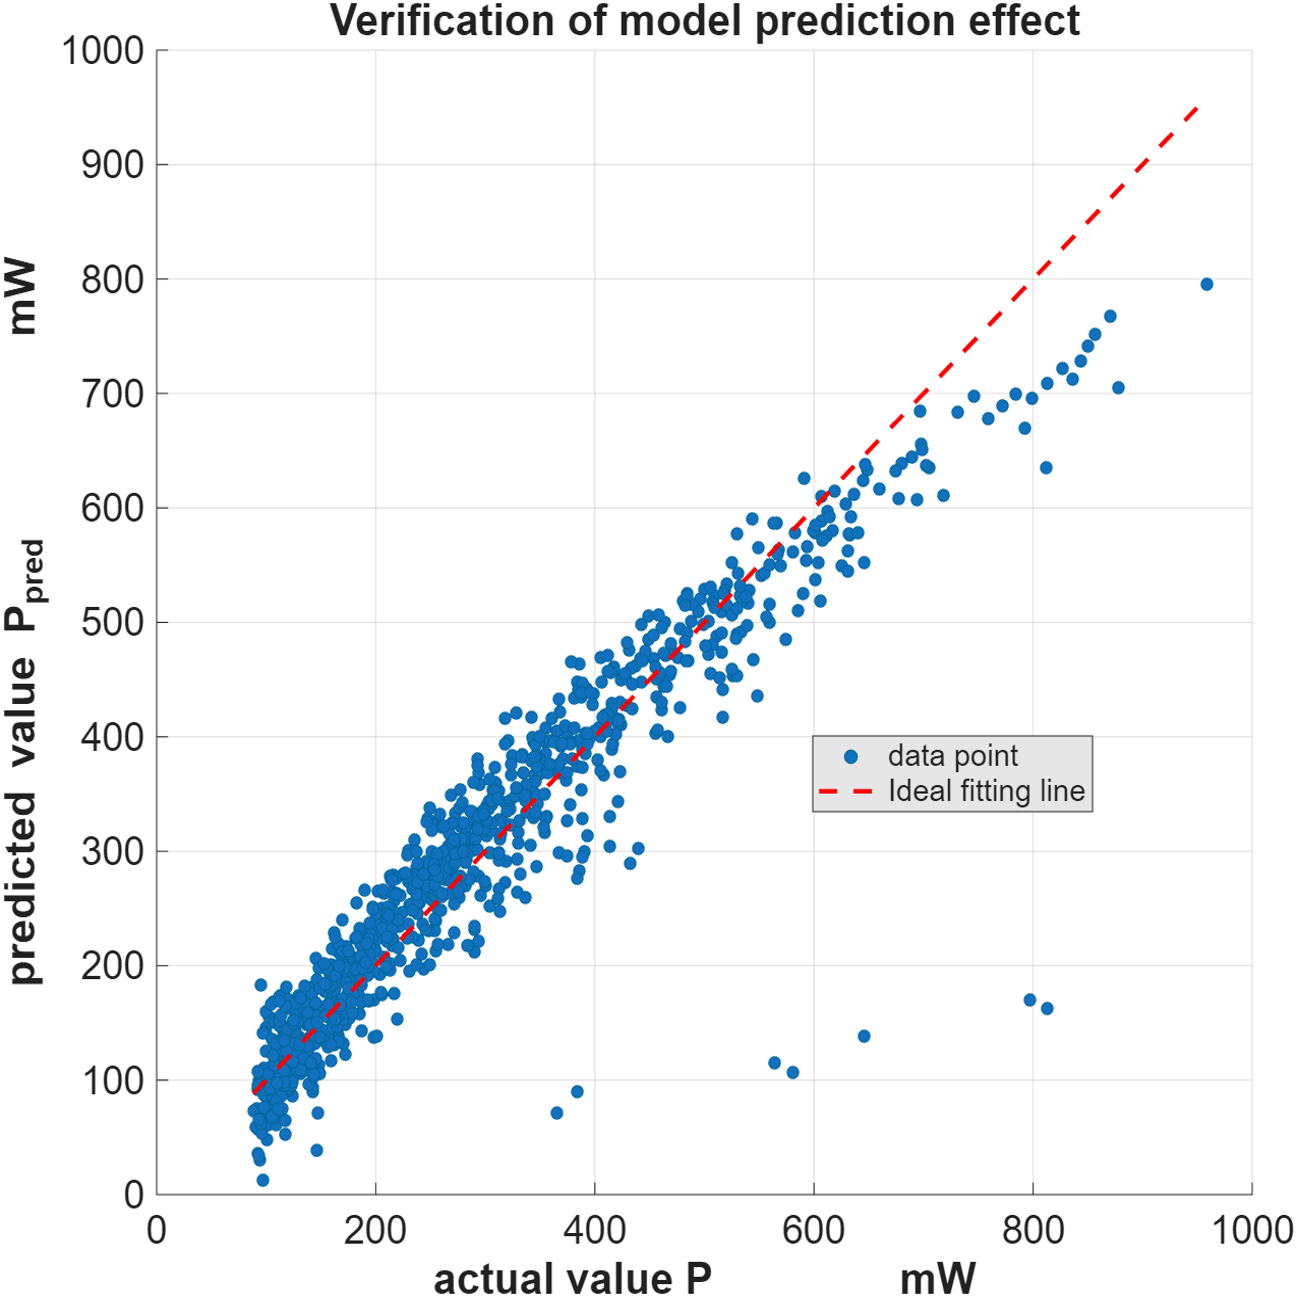
\includegraphics[width=0.6\textwidth]{verification.png}
	\caption{Comparison between Simulated Power and Measured Power}
	\label{fig:force_here}
\end{figure}

By calculation, we have a correlation coefficient of 0.938\,2, indicating a strong positive correlation between the simulated and measured power values. This preliminary validation suggests that our model is to some extent accurate in predicting smartphone battery consumption.

\section{Factor and Sensitivity Analysis}

\quad \, In this section, we analyze the influence of different factors. The method is to completely remove one factor out of the model, and simulate the battery drainage over one cycle again. Then the results are compared with the original simulation under 298 K. 

\begin{figure}[H]
	\centering
	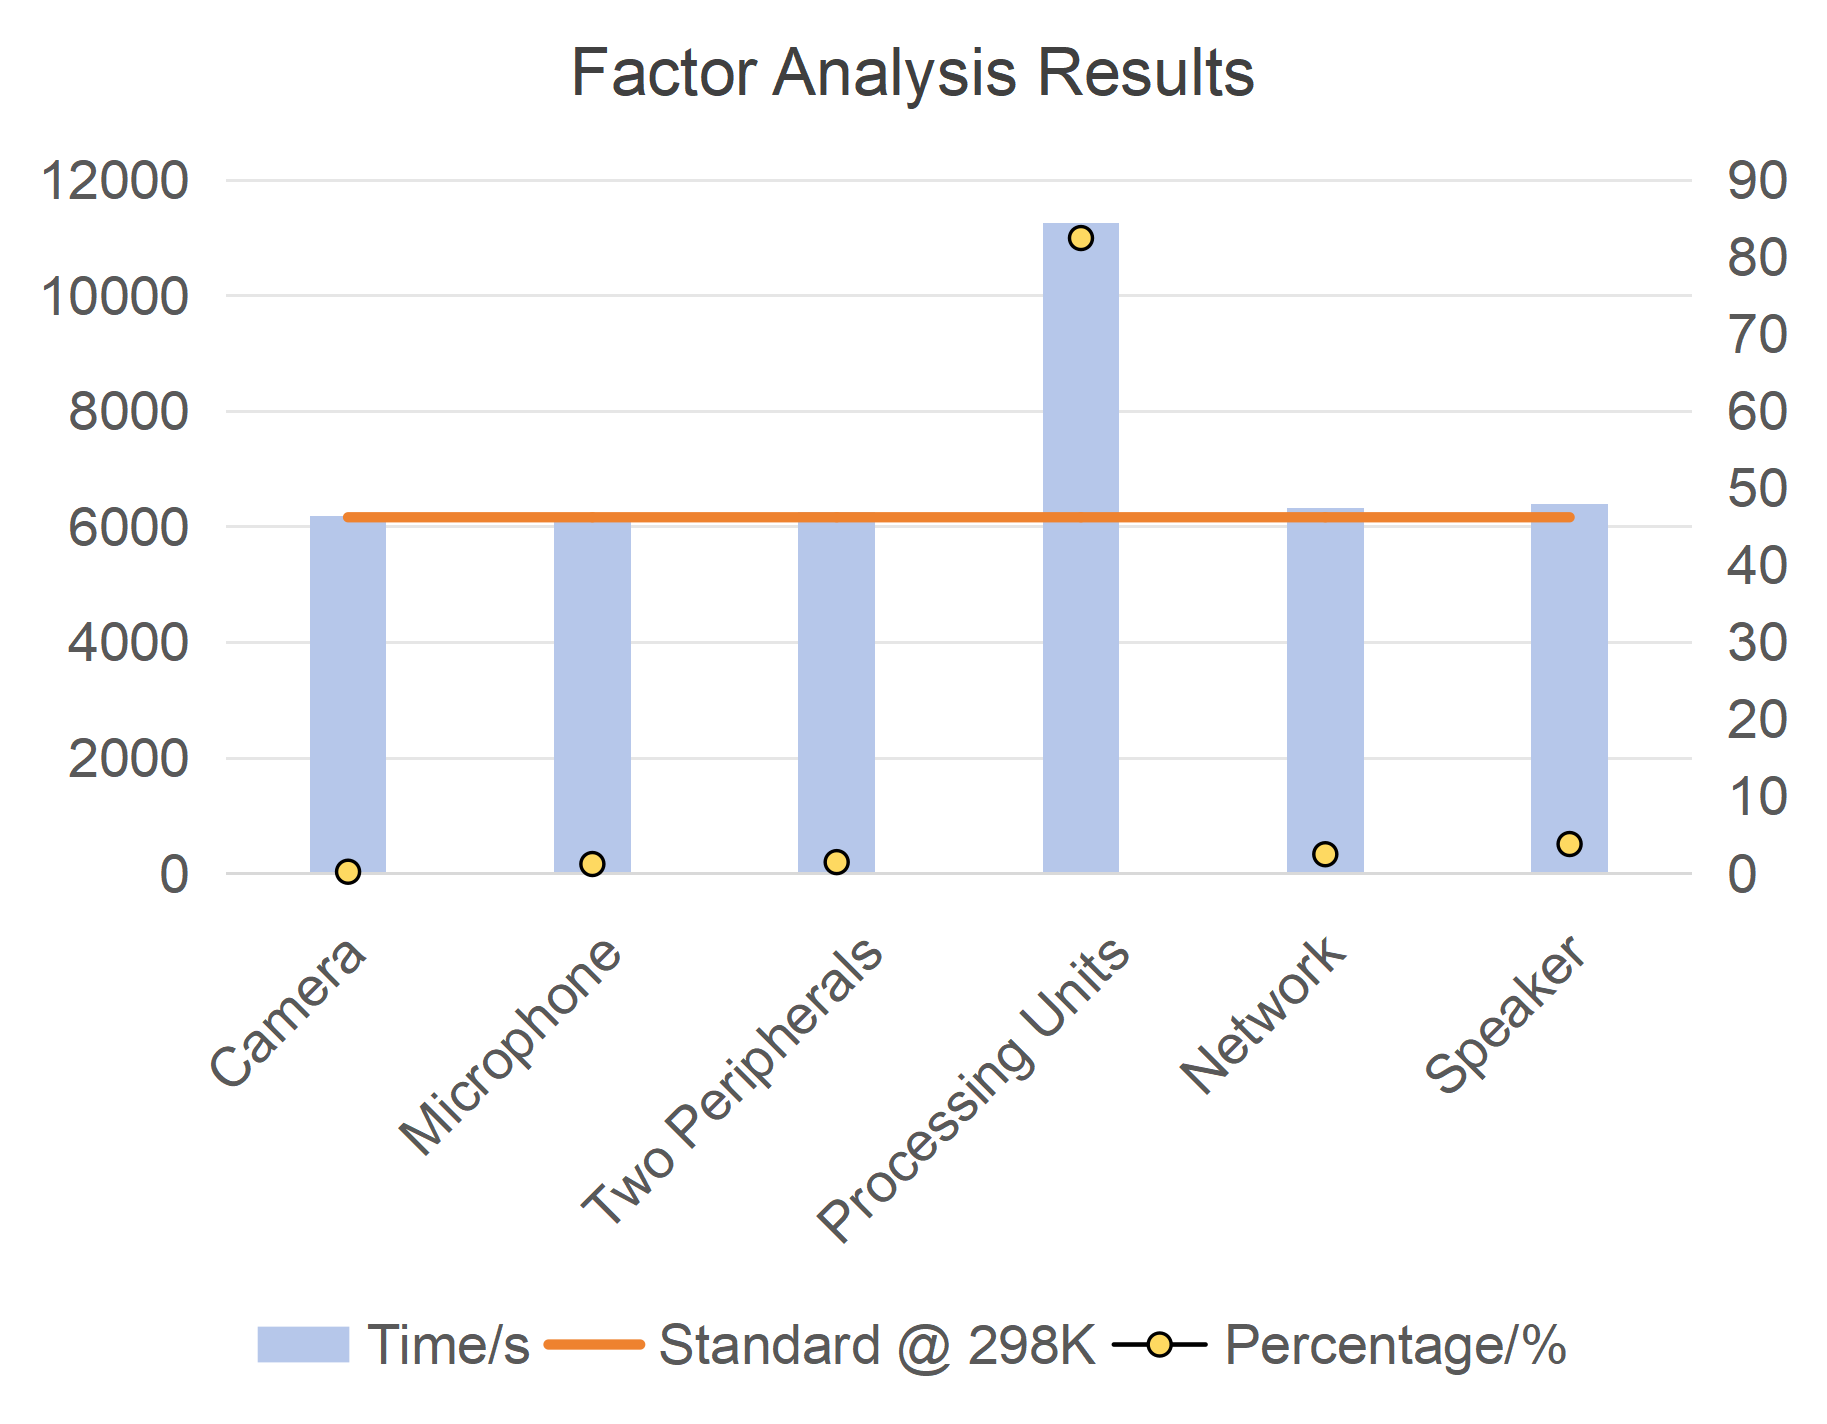
\includegraphics[width=0.6\textwidth]{Factor Analysis Results.png}
	\caption{Factor Analysis Results}
	\label{fig:force_here}
\end{figure}

The relevant data are listed below.

\begin{center}
\begin{tabular}{c|cc}
	\hline
	Factor Removed & Shutdown Time & Increase in Shutdown Time (\%) \\
	\hline
	None & 6\,166.2 & 0.000\,0 \\
	Camera & 6\,181.4 & 0.246\,5 \\
	Microphone & 6\,243.0 & 1.245\,5 \\
	Two Preipherals & 6\,258.2 & 1.492\,0 \\
	Processing Units & 11\,252.3 & 82.483\,5 \\
	Network & 6\,321.4 & 2.516\,9 \\
	Speaker & 6\,403.0 & 3.840\,3 \\
	\hline
\end{tabular}
\end{center}

From the results above one can clearly see that, apart from the processing units, the speaker factor has the most significant impact on battery drainage patterns, which comes quite unprecedented. After that is the network factor. The two peripherals have relatively minor effects on battery drainage patterns.

Apart from the factor analysis above, we also perform a sensitivity analysis on ambient temperature. The results are shown below.

\begin{figure}[H]
	\centering
	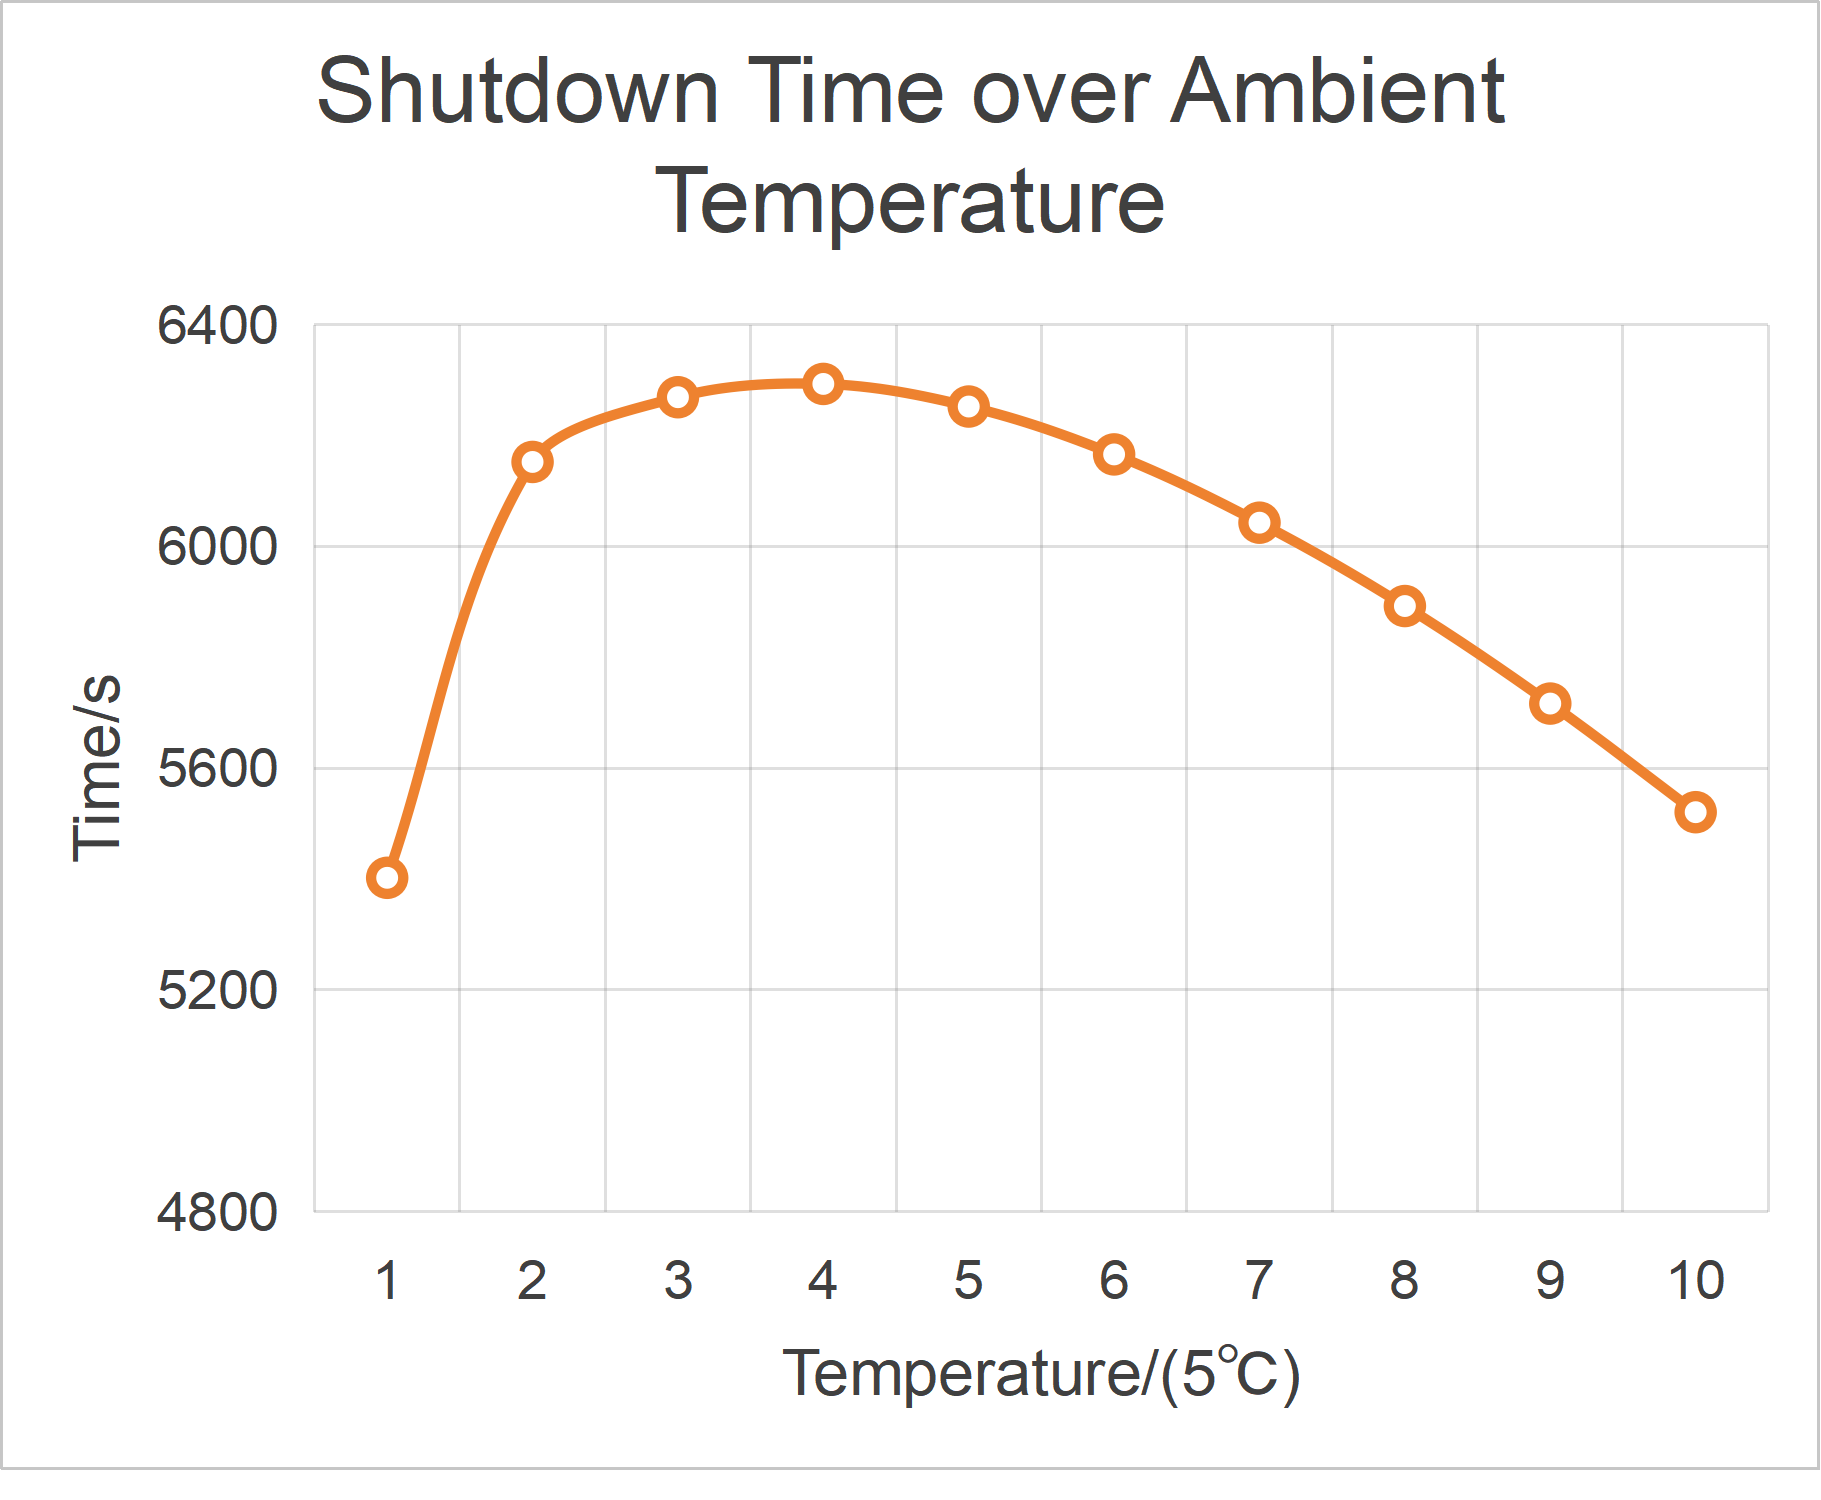
\includegraphics[width=0.6\textwidth]{Shutdown time over temp.png}
	\caption{Sensitivity Analysis on Ambient Temperature}
	\label{fig:force_here}
\end{figure}

The relevant data are listed below.

\begin{center}
\begin{tabular}{c|c}
	\hline
	Ambient Temperature ($^\circ$C) & Shutdown Time \\
	\hline
	0 & 5\,402.2 \\
	5 & 6\,152.6 \\
	10 & 6\,269.4 \\
	15 & 6\,293.4 \\
	20 & 6\,252.6 \\
	25 & 6\,166.2 \\
	30 & 6\,043.0 \\
	35 & 5\,892.6 \\
	40 & 5\,716.6 \\
	45 & 5\,520.6 \\
	\hline
\end{tabular}
\end{center}

One can see, that under extreme temperatures (both high and low), the battery drains much faster. The optimal ambient temperature for battery life is somewhere around 20$^\circ$C.

In terms of other parameters, one can clearly see from a mathematical point of view, that all equations regarding exponential functions are more sensitive to changes. Thus, we conclude that parameters in those equations are more sensitive. This includes parameters in Eq.(1), Eq.(4), Eq.(7), Eq.(20), Eq.(40), and Eq.(42): $E_\mathrm{a1}, E_\mathrm{a2}, c_2, c_4, \mathcal E^{\circ}_+, U_\mathrm{min+}, U_\mathrm{min-}, n, x$. As for other parameters, they are relatively less sensitive.

\section{Model Strengths and Weaknesses}

\subsection{Strengths}

\begin{enumerate}
	\item \textbf{Comprehensive Consideration of Factors:} Our model takes into account a wide range of factors that influence smartphone battery consumption, including screen usage, processing units, network activity, speakers, peripherals, thermal effects, and battery degradation. This comprehensive approach allows for a more accurate representation of real-world battery behavior.
	\item \textbf{Theoretical Foundation:} The model is built upon established physical and chemical principles, such as the Arrhenius equation, Nernst equation, and Fourier's law. This theoretical foundation enhances the credibility and reliability of the model.
	\item \textbf{Incorporation of Empirical Data:} Where necessary, the model incorporates empirical data and findings from previous scholarly works. This integration of empirical evidence helps to validate the theoretical aspects of the model and improve its accuracy.
\end{enumerate}

\subsection{Weaknesses}

\begin{enumerate}
	\item \textbf{Data Limitations:} The accuracy of our model is heavily dependent on the quality and quantity of the data used for calibration and validation. Limited or biased data can lead to inaccuracies in the model's predictions.
	\item \textbf{Simplified Assumptions:} To make the model tractable, we have made several simplifying assumptions, such as neglecting certain minor factors affecting battery performance. These assumptions may limit the model's applicability in real-world scenarios where these factors play a significant role.
	\item \textbf{Dynamic Usage Patterns:} The model may not fully capture the dynamic and complex usage patterns of smartphone users, which can lead to discrepancies between predicted and actual battery performance.
	\item \textbf{Theoretical Limitations:} While we have incorporated various physical and chemical principles into our model, there may still be theoretical limitations in our understanding of battery behavior that could affect the model's accuracy, due to our limited knowledge in chemistry and physics.
\end{enumerate}

\section{Practical Recommendations}

\subsection{OEMs}

\begin{enumerate}
	\item Improvements in battery chemistry can significantly enhance battery life. 
	\item Optimize CPU and GPU architectures for energy efficiency. For example, implementing performance and efficient core designs, dynamic voltage distribution between cores, even between CPU and GPU, can help reduce power consumption during high-load tasks.
	\item Reuse heat generated by components. One is easy to think of the Thomson effect and the Seebeck effect, which uses semi-conductors to convert temperature differences directly into electricity. 
	\item Update device firmwares and drivers. Ensure that the latest firmwares and drivers utilize the unique features of the hardware to cut power consumption.
\end{enumerate} 

\subsection{Operating System Developers}

\quad \, Here we mostly consider the network factor, which leads us to the following recommendations.

\begin{enumerate}
	\item Optimize background app network usage. If not necessary, postpone background network activities. 
	\item Provide user controls for network usage. Allow users to customize preferences for network-intensive activities, such as limiting data usage for specific apps when the battery is low.
	\item Optimize data transmission protocols. Use more efficient data compression and transmission techniques to reduce the amount of data sent and received.
\end{enumerate}

Apart from network, OS developers can also optimize CPU and GPU scheduling to reduce power consumption during high-load tasks. 

\subsection{App Developers}

\begin{enumerate}
	\item Reduce usages in peripherals. For example, avoid unnecessary camera and microphone usage in the background.
	\item Optimize algorithms. For example, some algorithms can be replaced with less accurate ones (still within acceptable error margins) that consume less power.
	\item Reduce network usage. Minimize data transmission by optimizing data synchronization and caching strategies. Moreover, cut all hidden uncensored and unnotified data collection and transmission. 
	\item Categorize computation loads. One may categorize loads into those suitable for CPU and those for GPU, and allocate them accordingly to optimize power consumption.
\end{enumerate}

\subsection{End Users}

\begin{enumerate}
	\item Cut all unnecessary background processes. This may be done by system settings, avoiding installing unnecessary apps, and avoiding authorizing unnecessary permissions.
	\item Adjust screen brightness and timeout settings. Lowering screen brightness and reducing the screen timeout duration can significantly decrease power consumption.
	\item Use power-saving modes. Most smartphones have built-in power-saving modes that limit background activities and reduce performance to extend battery life.
	\item Avoid extreme temperatures. Keep the smartphone within recommended temperature ranges to prevent accelerated battery degradation.
	\item Optimize charging habits. Avoid frequent complete discharges and overcharging to prolong battery lifespan.
\end{enumerate}

\section{Works Cited}

\noindent [1] Yang, S. et al. "Preferred LCD and OLED Luminance In Daily Tasks Is Affected By Ambient Lighting and Age". \textit{International Conference on Display Technology} \textbf{2021}, 2, 93-96. https://doi.org/10.1002/ sdtp.15029

\noindent [2][4][10] Bhat, G. et al. "Per-Core Power Modeling for Heterogenous SoCs". \textit{Energy} \textbf{2021}, 10, 2428.

\noindent [3][9] Huang, J. et al. "A Close Examination of Performance and Power Characteristics of 4G LTE Networks". \textit{Proceedings of the 10th international conference on Mobile systems, applications, and services}, 225–238. https://doi.org/10.1145/2307636.2307658

\noindent [5] Bouchet, S. et al. "Quantifying Loudspeakers' Power Consumption". \textit{Journal of the Audio Engineering Society} \textbf{2022}, 7/8, 601-610. 

\noindent [6] Chen, L. et al. "Estimation the Internal Resistance of Lithium-Ion Batteries Using a Multi-Factor Dynamic Internal Resistance Model with an Error Compensation Strategy". \textit{Energy Reports} \textbf{2021}, 7, 3050-3059.

\noindent [7] Yanase, T. et al. "Photoelectron Spectroscopy of Molecular Anion of Alq3: An Estimation of Reorganization Energt for Electron Transport in the Bulk". \textit{ACS Omega} \textbf{2018}, 3, 15200-15204.

\noindent [8] Paul, S. et al. "The Effect of Purcell Cavities on the Lifetime of Thermally Activated Delayed Fluorescence Emitters". \textit{Advanced Functional Materials} \textbf{2026}. https://doi.org/10.1002/adfm.202522114

\noindent [11] Haynes, W. M. et al, "CRC Handbook of Chemistry and Physics", 97th Edition, CRC Press, Boca Raton, FL, 2016-2017.
\\
\par Other Online Resources Used:

\noindent [12] "Specs of \textit{Google Pixel 8}" (translated) https://detail.zol.com.cn/1773/1772430/param.shtml

\noindent [13] Guegain, E. et al. "AndroWatts: Unpacking the Power Consumption of Mobile Device's Components". https://zenodo.org/records/14314943

\newpage

\section{Report on Use of AI}

\begin{enumerate}
	\item Baidu Fanyi, \textit{Baidu Translate} (Dec 9, 2025 version)\\
	Used for translating English terminologies into Chinese, and vice versa. 
	\item GitHub \textit{CoPilot} (Latest version) \\
	Auto-completion for code used in preparing our models.
\end{enumerate}

% Alas, the writer has gone for toilet. So this paper is handled to aliens. 

% ??? I thought of a brilliant proof, but here is no enough blank left. 

% HAHAHA I AM BACK, MOTHERFUCKERS.

%%%%%%%%%%%%%%%%%%%%%%%%%%%%%%
\end{document}
\end